\section{Results}\label{sec:results}

\subsection{The one-dimensional test (P1, P2)}\label{sec:beamres}
\paragraph{Uniform invariance.} Rotating every ply of the symmetric beam uniformly to
$20^\circ$ or $45^\circ$ lowers the linear frequency to $\nBUnifFTwenty$ and $\nBUnifFFortyFive$ of the
UD value ($\nBUDf$\,Hz). On the full FE model, the cubic SSM detuning coefficient is
unchanged to four digits (ratio $\nBUnif$), as Corollary~\ref{cor:beaminv} requires.
No uniform single-ply angle can therefore change $J$ at all.

\paragraph{Steering.} Table~\ref{tab:beam} and Fig.~\ref{fig:beam} report the optimized
symmetric beams. Every design has $\bm B\equiv\bm 0$, so the bending--extension
coupling plays no role. The optimizer does exactly what Proposition~\ref{prop:beam}
predicts: it turns the fibers off-axis in two zones centered, to within the knot spacing of the
angle field ($x/L=0.25$, $0.75$), on the inflection points ($x/L=0.224,0.776$), where $\varphi''^2$ vanishes, and keeps them axial where the beam
bends (Fig.~\ref{fig:beam}b). The SSM of the full FE beam confirms the condensed
evaluator's prediction for every design to within $\nBeamCondFE$ in $J/J_{\UD}$.
\begin{itemize}[itemsep=1pt]
\item \textbf{Tow-curvature limits.} At the $900^\circ$/m limit and $\omega_1\ge0.98\,
  \omega_{1,\UD}$, the detuning falls by $\nBNineHeldRed\%$. At $1800^\circ$/m it falls
  by $\nBEighteenHeldRed\%$, and with no tow limit by $\nBInfHeldRed\%$.
\item \textbf{Frequency allowance.} Relaxing the frequency to $0.90\,\omega_{1,\UD}$ gives
  $\nBNineNinetyRed\%$, $\nBEighteenNinetyRed\%$ and $\nBInfNinetyRed\%$ respectively.
\item \textbf{The coupling alternative.} The intuitive alternative is an unsymmetric
  laminate whose bending--extension coupling $\bm B(x)$ injects a softening quadratic
  force. We optimize it with its own, related objective (the RMS backbone drift over
  $a/h\le0.4$; two independently steered plies with two sine modes each, the same tow
  limit, and $\omega_1\ge0.90\,\omega_{1,\UD}$). It reduces that drift by only
  $\nBBred\%$, at $\nBBf\,\omega_{1,\UD}$. The comparison is therefore not like-for-like in
  objective, but the gap (a few percent against $\nBNineNinetyRed\%$ for symmetric steering at the same $900^\circ$/m limit and frequency floor) is far larger than the
  difference between the two objectives.
\end{itemize}
The lever on a clamped beam is therefore the spatial separation of curvature and
stretch, \emph{not} the bending--extension coupling. Its size is set by how narrow the
compliant zones can be (Corollary~\ref{cor:bang}). With no tow limit the two zones are each
$\approx0.05L$ wide at near-transverse fibers (total compliant length $\ell\approx0.1L$), and
\eqref{eq:bang} gives
$J/J_{\UD}\approx0.4$--$0.5$, against the computed $\nBInfHeld$. At $900^\circ$/m a
$90^\circ$ turn needs a third of the span, so the zones cannot both be narrow and
reach low modulus. This is why that limit binds.

\begin{table}[!tbp]
\centering\footnotesize
\caption{Symmetric steered beam: detuning ratio $J/J_{\UD}$ from the condensed evaluator
(optimizer) and from the full FE + cubic SSM (confirmation), with the realized frequency
ratio.}\label{tab:beam}
\begin{tabular}{@{}lcccc@{}}
\toprule
tow limit & frequency floor & $J/J_{\UD}$ condensed & $J/J_{\UD}$ FE+SSM & $\omega_1/\omega_{1,\UD}$ (SSM)\\ \midrule
$900^\circ$/m & $0.98$ & $\nBNineHeldCond$ & $\nBNineHeld$ & $\nBNineHeldf$\\
$900^\circ$/m & $0.90$ & $\nBNineNinetyCond$ & $\nBNineNinety$ & $\nBNineNinetyf$\\
$1800^\circ$/m & $0.98$ & $\nBEighteenHeldCond$ & $\nBEighteenHeld$ & $\nBEighteenHeldf$\\
$1800^\circ$/m & $0.90$ & $\nBEighteenNinetyCond$ & $\nBEighteenNinety$ & $\nBEighteenNinetyf$\\
none & $0.98$ & $\nBInfHeldCond$ & $\nBInfHeld$ & $\nBInfHeldf$\\
none & $0.90$ & $\nBInfNinetyCond$ & $\nBInfNinety$ & $\nBInfNinetyf$\\
\bottomrule
\end{tabular}
\end{table}

\begin{figure}[!tbp]
\centering
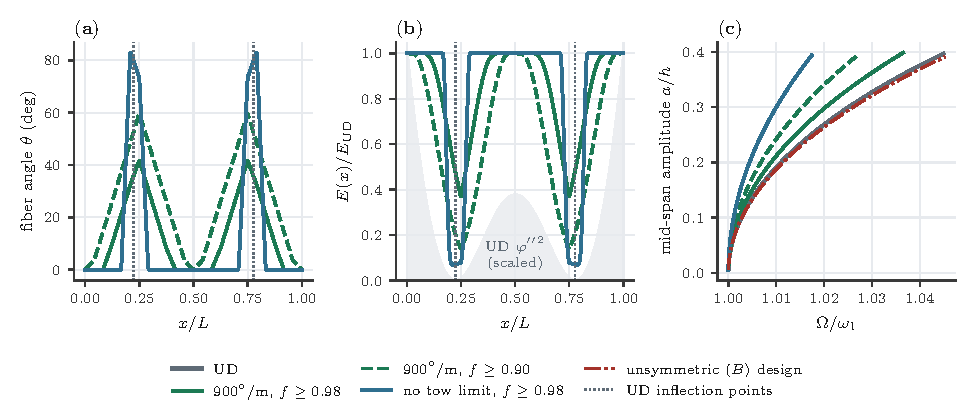
\includegraphics[width=\linewidth]{figs/fig_beam.pdf}
\caption{\textbf{On a symmetric beam, steering flattens the backbone by turning the fibers compliant
where the beam does not bend.} \textbf{(a)}~Optimized mirror-symmetric fiber angle
of the symmetric ($\bm B=\bm0$) clamped beam for three designs: tow limit $900^\circ$/m
with the frequency held to $f\geq0.98$ or $f\geq0.90$ of the UD value, and no tow limit
with $f\geq0.98$. The UD beam ($\theta\equiv0$, $E=E_{\UD}$) appears in (c) only.
\textbf{(b)}~The axial modulus these fields produce, against the UD curvature weight
$\varphi''^2$ that sets $\omega_1^2$ (shaded). Fibers turn compliant where the beam does
not bend: the inflection points (dotted). \textbf{(c)}~Mid-span backbones from the full FE
beam and its cubic SSM; steering flattens the backbone markedly. (The optimized
unsymmetric, $\bm B$-coupled laminate was computed on a different beam model and objective,
so it is compared in the text, not plotted.)}
\label{fig:beam}
\end{figure}

\subsection{The achievable frequency--hardening set of the plate (P3)}\label{sec:levers}
Figure~\ref{fig:levers}a places every design class in the plane
$(\omega_1/\omega_{1,\UD},\,J/J_{\UD})$ at the same mass.

\paragraph{Uniform layups.} A uniform single angle traces a one-parameter curve. As
$\theta$ grows from $0^\circ$ the plate stiffens (up to $\nUfmax\,\omega_{1,\UD}$ at
$90^\circ$, fibers across the short span), and $J$ first falls to $\nUJmin$ at
$\theta=\nUthJmin^\circ$, where $\omega_1=\nUfatJmin\,\omega_{1,\UD}$, then rises. The
$\nSnum$ uniform symmetric stacks on a $15^\circ$ grid fill a region with a global
minimum of $\nSmin$ at $\nSfatmin\,\omega_{1,\UD}$. A grid envelope is not the strongest
uniform competitor: between grid points the continuous single angle already beats it
($\nUEleven$ vs.\ $\nGEleven$ at $1.1\,\omega_{1,\UD}$). We therefore also optimize the
four ply angles of $[\theta_4/\theta_3/\theta_2/\theta_1]_s$ \emph{continuously} at each
held frequency (SLSQP with the frequency equality, 22 starts from the best grid stacks,
the single-angle solution and random stacks; \texttt{stack\_continuous.py}). The best
uniform laminate reaches $J/J_{\UD}=\nCSEleven$, $\nCSTwelve$ and $\nCSThirteen$ at
$1.1$, $1.2$ and $1.3\,\omega_{1,\UD}$.

\paragraph{The UD floor.} Corollary~\ref{cor:udfloor} proves that the lowest-frequency uniform
symmetric laminate of this plate is a single-angle one, and the single-angle sweep shows that it is
UD. The enumeration agrees: the smallest stack frequency is $\nSfmin\,\omega_{1,\UD}$. At
exactly $\omega_1=\omega_{1,\UD}$ the continuous stack optimum is UD itself (all ply angles
$\to0$); the best grid stack within $\pm1\%$ of that frequency, at a slightly different
$\omega_1$, has $J/J_{\UD}=\nSheld$, a negligible difference. For a plate
mandated to the UD frequency, the uniform design space is therefore a single point. This is the one
comparison that is exact for \emph{every} uniform laminate. Above $\omega_{1,\UD}$ the uniform
competitors are the classes we surveyed: all single angles, all $\nSnum$ grid stacks and the
continuously optimized eight-ply stacks. Those comparisons are numerical, not proved bounds.

\paragraph{Steered designs.} At exactly $\omega_{1,\UD}$, the steered single ply reaches
$J/J_{\UD}=\nFTen$, a $\nFTenRed\%$ reduction, with $R_{\min}=\SI{20}{mm}$ imposed (it is active but changes $J$ only in the fourth digit: without
it the optimum is $\nResAInf$, Sec.~\ref{sec:limits}). The steered designs lie well below the best surveyed uniform laminate at
every frequency we test: $\nFEleven$, $\nFTwelve$ and $\nFThirteen$ at $1.1$,
$1.2$ and $1.3\,\omega_{1,\UD}$, against $\nCSEleven$, $\nCSTwelve$ and $\nCSThirteen$
for the best continuous stacks. Steering can also \emph{lower} the frequency below the uniform floor
($\nFNine$ at $0.9\,\omega_{1,\UD}$), which, by Corollary~\ref{cor:udfloor}, no uniform laminate can do. Steering the best
stack at $\omega_{1,\UD}$ gives $\nSFTen$, no better than the steered single ply. For
this plate and objective, the in-plane channel of Sec.~\ref{sec:channels} dominates the
through-thickness channel. Prediction P3 holds with a wide margin: exactly at $\omega_{1,\UD}$,
and against every surveyed uniform class above it.

\begin{figure}[!tbp]
\centering
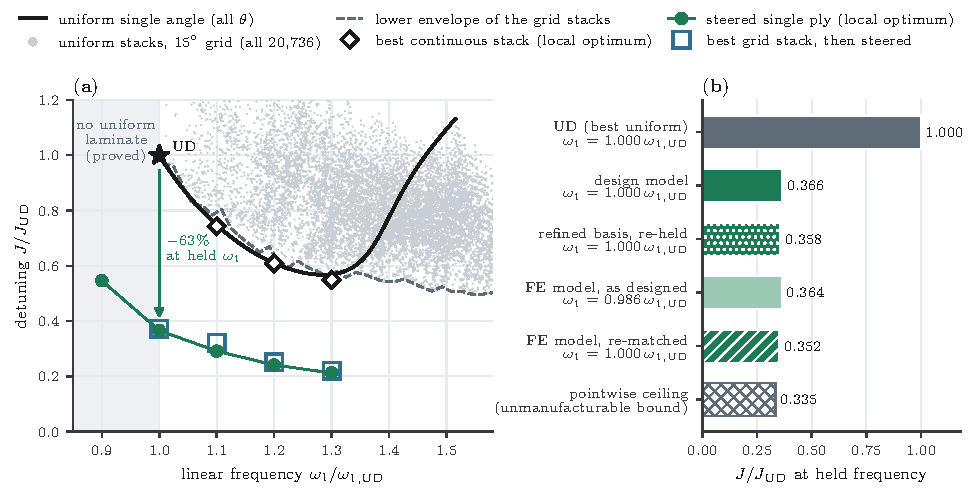
\includegraphics[width=\linewidth]{figs/fig_levers.pdf}
\caption{\textbf{At the unidirectional frequency and mass, steering reaches a hardening that no uniform
symmetric laminate can reach, and above it steering undercuts every uniform class surveyed; the
held-frequency result holds with the frequency re-matched in every model.} \textbf{(a)}~Linear
frequency vs.\ frequency-normalized hardening. Provenance is marked in the legend.
\emph{Proved}: the shaded band $\omega_1<\omega_{1,\UD}$, where no uniform laminate exists
(Corollary~\ref{cor:udfloor}). \emph{Exhaustive}: the uniform single angle (black curve) and all
$\nSnum$ symmetric stacks on a $15^\circ$ grid (gray dots, clipped at $J/J_{\UD}=1.2$; dashed: their
lower envelope). \emph{Local optima}: the best continuous eight-ply stack at each held frequency
(open diamonds, 22 starts), the steered single ply at five target frequencies with
$R_{\min}=\SI{20}{mm}$ (green), and the best grid stack at each target, then steered (blue squares;
none exists at $0.9\,\omega_{1,\UD}$). The arrow marks the held-frequency reduction.
\textbf{(b)}~The held-frequency design's $J/J_{\UD}$ in each model, with the frequency at which it
is evaluated: the design model (equality exact); a refined basis ($m,n\le12$) with the equality
re-imposed; the independent FE model as designed ($\omega_1$ $\nHeldTol\%$ low) and with the
frequency re-matched; the full multi-mode plate's SSM as designed ($\omega_1$ $\nFullAsisPct\%$ high) and
re-matched; and the pointwise ceiling of Sec.~\ref{sec:limits} (unmanufacturable; an estimate). At
$\omega_{1,\UD}$ the best uniform laminate is UD itself; the best grid stack there is UD to within
$\nGridStackDiff\%$ in $J$ ($[0/0/0/15]_s$), and steering it gives $\nSFTen$.}
\label{fig:levers}
\end{figure}

\subsection{The mechanism (P4)}\label{sec:mechanism}
Figure~\ref{fig:mechanism} tests the mechanism of Sec.~\ref{sec:theory} directly.
\begin{itemize}[itemsep=1pt]
\item \textbf{Where the energies live.} Both energies of the UD mode peak at the center.
  The bending energy is concentrated there, with the principal curvature along $y$, across
  the short span, so the held-frequency constraint favors fibers along $x$ there (panel a). The relaxed-stretch energy lies in a band along $x$ through
  the center, with its across-stretch direction along $x$ there and turning toward the
  corners (panel b).
\item \textbf{Sign of the trade-off.} At the held UD frequency the multiplier is negative,
  $\Lambda=\nLambda$ (dimensionless: $e_G$ and $e_K$ normalized by the UD $\gamma$ and
  $\omega_1^2$): minimizing the stretch energy alone would raise the frequency to
  $\nFreeFreq\,\omega_{1,\UD}$, so the constraint pushes the fibers \emph{across} the
  curvature. At the center the two preferences agree (fibers along $x$), and the pointwise design
  $\theta^\star$ keeps the UD direction there.
\item \textbf{Conflict.} Away from the center the across-stretch and across-curvature
  directions separate (panel c); their energy-weighted mean angle is $\nConflict^\circ$.
  This is where a single angle must compromise.
\item \textbf{Pointwise prediction.} The first-order design $\theta^\star(\bm x)$ of
  Proposition~\ref{prop:pointwise}, computed from the UD fields alone with no optimizer
  and no smoothness (panel d), already gives $J/J_{\UD}=\nStarJ$ when evaluated on the
  full model. Its frequency is $\nStarF\,\omega_{1,\UD}$, because the frozen-field model
  ignores the adaptation of the mode.
\item \textbf{Optimized field.} The optimized, curvature-limited field (panel e) shares the
  large-scale pattern of $\theta^\star$ (fibers turned off-axis toward the short edges) but
  departs from it in detail: the energy-weighted RMS angle difference is $\nStarDev^\circ$
  over the plate and $\nStarDevHigh^\circ$ where the energies are large, and at the energy
  peak the optimum is tilted to $\nOptAtPeak^\circ$. The frozen-field design ignores the
  adaptation of the mode and the smoothness and tow limit of a curvature-feasible field, both
  of which the optimizer must respect.
\end{itemize}

Panel f shows which terms move, normalized by UD:
\begin{itemize}[itemsep=1pt]
\item the raw (restrained) membrane cubic falls to $k_{nl}=\nDknl$;
\item the relaxation $2\bm g^{\!\top}\bm K_{\mathrm{in}}^{-1}\bm g$ changes to $\nDrelax$ of
  its UD value, a share of $k_{nl}$ rising from $\nRelaxUD\%$ to $\nRelaxOpt\%$;
\item the relaxed cubic falls to $\gamma=\nDgamma$;
\item the frequency is held ($\omega_1^2=\nDomsq$) and the mode's center value changes to
  $w_c=\nDmid$.
\end{itemize}
The hardening falls mainly through the direct term of \eqref{eq:gamma}: fibers across the
principal stretch store less membrane energy for the same stretch, so $k_{nl}$ falls to
$\nDknl$ of its UD value. The relaxation falls less (to $\nDrelax$), so its share of the
stretch energy rises and $\gamma$ falls further than $k_{nl}$ alone. Prediction P4 holds
partly: $\theta^\star$ alone captures most of the gain, though at $\nStarF\,\omega_{1,\UD}$, but the optimum departs from it by $\nStarDevHigh^\circ$ RMS even where the
energies are large.

\begin{figure}[!tbp]
\centering
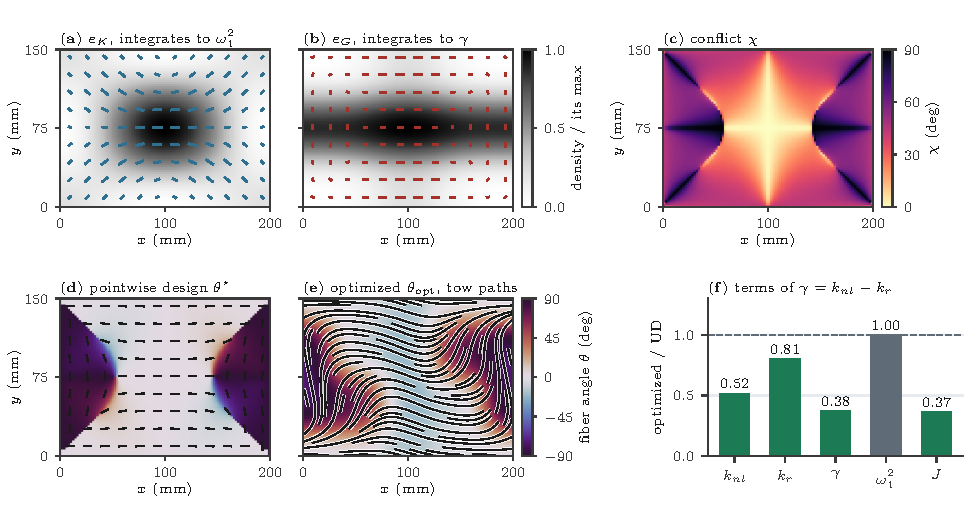
\includegraphics[width=\linewidth]{figs/fig_mechanism.pdf}
\caption{\textbf{The two energies prefer different fiber directions away from the plate
center; the optimized field follows a compromise that a single angle cannot make.} All maps show the
full $\SI{200}{mm}\times\SI{150}{mm}$ plate with the same axes; angles are measured from the $x$
axis. \textbf{(a)}~Bending-energy density $e_K$ of the UD fundamental, which integrates to
$\omega_1^2$. Blue ticks: the fiber direction the held-frequency constraint favors ($\Lambda<0$:
across the principal curvature, $\varphi_K+90^\circ$). \textbf{(b)}~Relaxed-stretch density $e_G$,
which integrates to $\gamma$, on the same normalized gray scale. Red ticks: the direction that
minimizes it (across the principal stretch, $\varphi_G+90^\circ$). Tick length in (a) and (b)
scales with the local anisotropic amplitude. \textbf{(c)}~Conflict $\chi$, the angle between the
ticks of (a) and (b). It vanishes at the center and along the central cross ($x=\SI{100}{mm}$, and
$y=\SI{75}{mm}$ for $60<x<\SI{140}{mm}$), where one direction serves both energies, and reaches $90^\circ$
along $y=\SI{75}{mm}$ near the short edges. The sharp ridges are lines where one of the two principal directions is undefined
(equal principal strains). \textbf{(d)}~First-order pointwise design $\theta^\star$ from the UD
fields alone (Proposition~\ref{prop:pointwise}); black ticks: the same direction field.
\textbf{(e)}~Optimized curvature-limited field; colors give the fiber angle and black lines the tow
paths. (d) and (e) share one cyclic color scale, lightest at $\theta=0^\circ$.
\textbf{(f)}~Optimized/UD ratios of the terms of \eqref{eq:gamma}: the restrained cubic $k_{nl}$,
the relaxation $k_{r}=2\bm g^{\!\top}\bm K_{\mathrm{in}}^{-1}\bm g$, their difference $\gamma$,
$\omega_1^2$ (held) and $J$; dashed: parity with UD.}
\label{fig:mechanism}
\end{figure}

\subsection{What bounds the lever (P5)}\label{sec:limits}
\paragraph{Anisotropy.} Along the family $\bm Q(s)=\bm Q_{\mathrm{iso}}+s(\bm Q-\bm
Q_{\mathrm{iso}})$, which keeps the isotropic invariants $U_1,U_4,U_5$ and scales $U_2,U_3$
by $s$, the held-frequency steered optimum falls monotonically with the anisotropy:
\begin{itemize}[itemsep=1pt]
\item $J/J_{\UD}=\nDoseA$ at $E_1/E_2=\nDoseRatioA$;
\item $\nDoseC$ at $\nDoseRatioC$;
\item $\nDoseE$ at $\nDoseRatioE$ (CFRP);
\item $\nDoseF$ at $\nDoseRatioF$ (Fig.~\ref{fig:limits}a).
\end{itemize}
The isotropic limit has no lever (Corollary~\ref{cor:iso}).

\paragraph{Tow curvature.} The held-frequency optimum degrades smoothly as the minimum
tow radius grows:
\begin{itemize}[itemsep=1pt]
\item $\nFrontThirty$ at $R_{\min}=\SI{30}{mm}$;
\item $\nFrontFifty$ at $\SI{50}{mm}$;
\item $\nFrontEighty$ at $\SI{80}{mm}$;
\item $\nFrontOneFifty$ at $\SI{150}{mm}$;
\item $\nFrontFourHundred$ at $\SI{400}{mm}$ (Fig.~\ref{fig:limits}b).
\end{itemize}
Below $R_{\min}\approx\SI{20}{mm}$ it saturates at $\nFrontTwenty$. Two checks show that
the saturation is physical rather than an artifact of the 50\,mm support grid.
\begin{itemize}[itemsep=1pt]
\item \textbf{Finer grid.} Refining the grid to 33\,mm and 25\,mm changes the optimum
  only to $\nResBTwenty$ and $\nResCTwenty$ at $R_{\min}=\SI{20}{mm}$, and to
  $\nResBInf$ and $\nResCInf$ with no tow limit.
\item \textbf{Pointwise ceiling.} Freeing $\theta$ at every quadrature point, with no
  smoothness and no tow limit, gives $\nCeil$. This field cannot be laid, and it is the best
  local optimum found for a nonconvex problem, so it estimates rather than bounds what
  single-ply steering can reach.
\end{itemize}
The plate's strain fields vary on a length scale of a few centimeters. Once tows can
turn on that scale, further manufacturing freedom buys little. The front of
Fig.~\ref{fig:limits}b is the best design found from six starts at each radius, so the attainable
front lies at or below it; the pointwise ceiling indicates how much lower it could plausibly go. Prediction P5 holds:
the lever is set by the material anisotropy and by the ratio of the tow radius to the
length scale of the mode's strain fields. Its third ingredient, the conflict between the two
fields, is tested across plates in Sec.~\ref{sec:robust}.

\begin{figure}[!tbp]
\centering
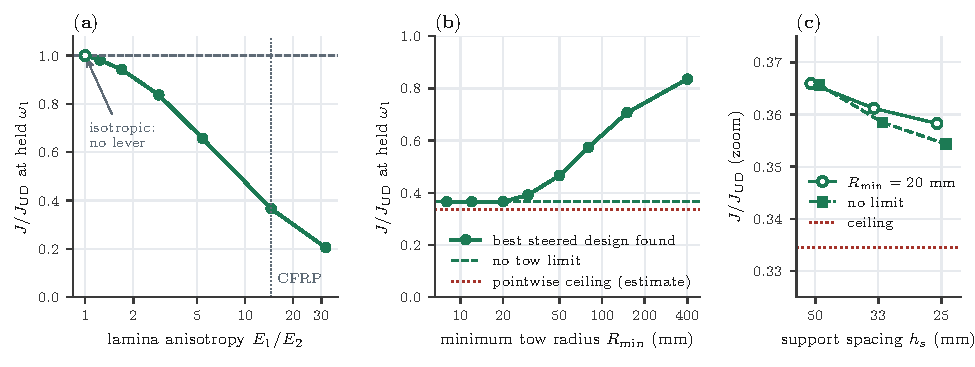
\includegraphics[width=\linewidth]{figs/fig_limits.pdf}
\caption{\textbf{The lever vanishes for isotropic material, grows with anisotropy, and saturates
once tows can turn on the strain-field length scale.} All at held frequency. \textbf{(a)}~Steered optimum vs.\
lamina anisotropy along a family that scales only the anisotropic invariants
($E_1/E_2=1$ is isotropic, where $J/J_{\UD}=1$ exactly by Corollary~\ref{cor:iso}, so that point is
not computed; dashed: parity with UD; dotted: CFRP). \textbf{(b)}~Tow-radius front: best design found vs.\ minimum tow
radius on the 50\,mm support grid; dashed: the same grid with no tow limit; dotted: the
pointwise ceiling (unconstrained, unsmoothed; an estimate, not a bound). Each point is the best of six
starts.
\textbf{(c)}~Support-grid refinement (zoomed
ordinate; the three support spacings are plotted as equally spaced categories, with the two
series offset slightly for visibility): at $R_{\min}=\SI{20}{mm}$ (open) and with no tow limit (filled) the optimum
moves by less than $0.02$ and approaches the ceiling, so the saturation in (b) is physical,
not a parametrization artifact.}
\label{fig:limits}
\end{figure}

\subsection{Independent confirmation on the full model}\label{sec:confirm}
The design was produced on the condensed, adapted-mode evaluator. We confirm it on the
full multi-mode plate: 36 transverse and 72 in-plane modes, in-plane inertia retained,
an independent Gauss-quadrature assembly, and amplitudes measured as the true mid-plate
deflection (Table~\ref{tab:confirm}).
\begin{itemize}[itemsep=1pt]
\item \textbf{Full SSM.} The full cubic SSM gives detuning coefficients $\beta$ within
  $\nSSMvsEval\%$ of the evaluator for both designs. The detuning ratio is $\nCratioSSM$, a
  $\nCredSSM\%$ reduction.
\item \textbf{EPMC.} Full-order EPMC continuation ($H=\nEPMCH$ harmonics) gives a ratio of $\nCratioEPMC$.
\item \textbf{Frequency.} The steered design's full-model frequency is $\nCOptf$\,Hz
  against $\nCUDf$\,Hz for UD. The difference is the Ritz upper-bound convergence of the
  transverse basis for the steered field (Table~\ref{tab:conv}: the steered frequency
  falls by $\nConvFreqDrop\%$ from $m,n\le8$ to $m,n\le16$ while the UD frequency is unchanged), not a
  design change.
\item \textbf{Discretization.} An independent finite-element model (ACM Kirchhoff
  bending with Q4 membrane elements, Appendix~\ref{app:fe}) evaluated on the optimized
  field gives a detuning ratio of $\nFEratio$. Across the three discretizations the
  steered design's frequency lies within $\pm\nHeldTol\%$ of the UD value.
\end{itemize}

\paragraph{Matched-frequency comparison.} In the refined design basis and in the FE model the steered
frequency comes out slightly \emph{below} the UD value, which is unfavorable to steering because $J$ falls
as the frequency rises along the steered front (Fig.~\ref{fig:levers}a). In the full multi-mode plate it
comes out $\nFullAsisPct\%$ \emph{above}, which favors it. To remove the drift in both directions rather
than bound it, we re-impose the equality in each model (\texttt{r1\_\allowbreak matched\_\allowbreak
frequency.py}, \texttt{r1\_\allowbreak full\_\allowbreak matched.py}; Fig.~\ref{fig:levers}b).
\begin{itemize}[itemsep=1pt]
\item \textbf{Refined basis.} On $m,n\le12$ (144 transverse and 128 in-plane modes) the published design
  has $\omega_1=\nRefEvalF\,\omega_{1,\UD}$ and $J/J_{\UD}=\nRefEvalJ$. Re-solving the held-frequency
  problem on that basis, with the equality exact, gives $J/J_{\UD}=\nRefHeldJ$.
\item \textbf{Independent FE model.} The design as laid has $\omega_1=\nFEasisF\,\omega_{1,\UD}$ and ratio
  $\nFEasisJ$. We move it along the design model's frequency-gradient direction until the FE
  frequencies agree to $10^{-5}$ (a one-parameter move, not a re-optimization, so conservative). The ratio
  is then $\nFEmatchedJ$. Along that path
  $\dd(J/J_{\UD})/\dd(\omega_1/\omega_{1,\UD})=-\nFEslope$, so a frequency drift of $1\%$ moves the
  headline ratio by less than $0.01$.
\item \textbf{Full multi-mode plate.} Moved in the same way until its linear frequency equals the UD
  value to $10^{-6}$, the steered design has an SSM detuning ratio of $\nFullMatchedJ$ (as designed:
  $\nCratioSSM$) and an EPMC ratio of $\nFullMatchedEPMC$.
\end{itemize}
The held-frequency result is therefore not an artifact of the design discretization. With the
frequency matched in each model, the steered plate is at $\nFEmatchedJ$--$\nFullMatchedEPMC$ of the UD
hardening.

\begin{table}[!tbp]
\centering\footnotesize
\caption{Confirmation of the held-frequency design. $\beta$: small-amplitude coefficient
of $\Om/\omega_1-1=\beta(a/h)^2$ at the plate center.}\label{tab:confirm}
\begin{tabular}{@{}lcccc@{}}
\toprule
model & $f_1$ UD (Hz) & $f_1$ steered (Hz) & $\beta$ UD & $\beta$ steered\\ \midrule
design evaluator (64+72 modes, condensed) & $\nUDf$ & $\nUDf$ & $\nEvBetaUD$ & $\nEvBetaOpt$\\
full plate, cubic SSM (36+72 modes) & $\nCUDf$ & $\nCOptf$ & $\nCUDbetaSSM$ & $\nCOptbetaSSM$\\
full plate, EPMC ($H=\nEPMCH$) & --- & --- & $\nCUDbetaEPMC$ & $\nCOptbetaEPMC$\\
independent FE (ACM + Q4, $\nFEmesh$, App.~\ref{app:fe}) & $\nFEUDf$ & $\nFEOptf$ & $\nFEUDbeta$ & $\nFEOptbeta$\\
\bottomrule
\end{tabular}
\end{table}

\subsection{Consequence: a wider jump-free range}\label{sec:jumpres}
The backbone improvement (Secs.~\ref{sec:levers}--\ref{sec:confirm}) is a property of the
conservative system. Turning it into a forced-response statement needs a damping model and a
forcing, so the absolute numbers below are specific to the model ($\zeta=2\%$ mass-proportional, a
center point load). The \emph{ratio} of jump-free amplitudes is not: Proposition~\ref{prop:cusp}
predicts that the held-frequency reduction widens the jump-free amplitude by
$(J_{\mathrm{steered}}/J_{\UD})^{-1/2}=\nCacTheory$, whatever $\zeta$ is, and
Sec.~\ref{sec:robust} tests that independence. We compute
$a_c$ numerically as the drive at which the full-order damped SSM forced response
($\zeta=2\%$, center point load) first becomes multivalued. It rises from $a_c/h=\nCUDac$
to $\nCOptac$, a factor $\nCacRatio$ in amplitude and $\nCFratio$ in drive. This agrees
with the predicted ratio, and the absolute thresholds agree too: \eqref{eq:ac} with the
full-model $\beta$ gives $\nCacFormUD$ and $\nCacFormOpt$.

Direct time integration then shows the jump itself (Fig.~\ref{fig:confirm}b,c). We drive
both panels with the same point load, set between their two thresholds, and sweep the
frequency up and down. The UD panel is hysteretic: the up and down sweeps differ by up
to $\nCUDgap\,h$ across the fold. The steered panel, at the same frequency and mass, is
single-valued: its sweeps coincide to $\nCOptgap\,h$ and follow the SSM forced response. A finer
sweep ($\nFineSteps$ steps over $\Om/\omega_1\in[1.00,1.08]$; \texttt{confirm\_\allowbreak fine\_\allowbreak sweep.py})
confirms both: the UD up and down sweeps differ at $\nFineHyst$ consecutive steps across the
fold (by up to $\nFineGap\,h$), the steered sweeps at none.
\begin{figure}[!tbp]
\centering
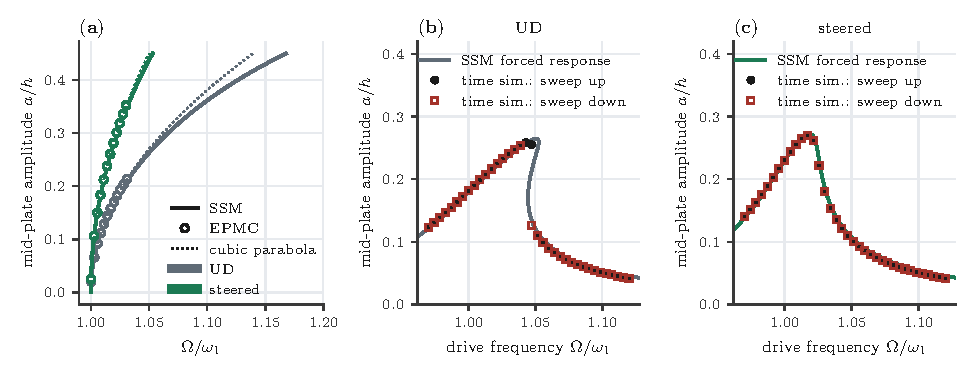
\includegraphics[width=\linewidth]{figs/fig_confirm.pdf}
\caption{\textbf{The full model confirms the reduction, and at one drive the UD panel jumps while the
steered panel, at the same frequency and mass, does not.} \textbf{(a)}~Free mid-plate backbones of the
full multi-mode plate (36 transverse + 72 in-plane modes): cubic SSM (lines) and full-order EPMC with
$H=\nEPMCH$ harmonics (marks; squares UD, circles steered). Dotted: the cubic parabola
$1+\beta(a/h)^2$ with the full-model SSM $\beta$ (within $\nSSMvsEval\%$ of the condensed evaluator's).
\textbf{(b,c)}~Forced response at one drive between the two jump thresholds ($\zeta=2\%$, center point
load): full-plate damped SSM (line) and direct time integration of up sweeps (black dots) and down sweeps
(red squares) on a six-mode modal model, 300 forcing periods per step. A point is kept once its
amplitude is steady to $0.4\%$, which excludes one UD point at the fold.}
\label{fig:confirm}
\end{figure}

\subsection{Robustness of the lever}\label{sec:robust}
The result above is for one plate, one support, one damping law and an idealized laminate. This
section varies each in turn (Fig.~\ref{fig:robust}).

\paragraph{Other plates and the conflict test of P5.} We solve the same held-frequency problem
($R_{\min}=\SI{20}{mm}$, 50\,mm support grid, six starts) for a square and a 2:1 plate, for clamped
edges, and for in-plane traction-free edges, and compare each with the strongest uniform laminate at
the same frequency (all single angles and a continuous eight-ply stack optimization;
\texttt{r1\_\allowbreak generality.py}).
\begin{itemize}[itemsep=1pt]
\item \textbf{Aspect ratio.} The steered optimum is $J/J_{\UD}=\nGenSqJ$ on the square plate and
  $\nGenTwoJ$ on the 2:1 plate, against $\nGenBaseJ$ on the paper's 4:3 plate. On all three the UD
  plate is again the lowest-frequency uniform laminate, so UD is the best uniform design at
  $\omega_{1,\UD}$.
\item \textbf{Clamped edges.} Here UD is \emph{not} the frequency floor: the lowest uniform frequency,
  $\nGenClMinF\,\omega_{1,\UD}$, occurs at a single angle of $\nGenClMinAng^\circ$, as
  Corollary~\ref{cor:udfloor} allows. A real uniform competitor therefore exists at $\omega_{1,\UD}$. It
  reaches $\nGenClUnif$, and the steered field reaches $\nGenClJ$.
\item \textbf{In-plane movable edges.} With traction-free in-plane edges the UD plate hardens
  $\nGenMvRatio$ times less, because $\nGenMvRelaxUD\%$ of its stretch energy relaxes. Steering still
  halves what remains ($\nGenMvJ$), raising the relaxed share to $\nGenMvRelaxOpt\%$.
\end{itemize}
The lever is general, but its size varies by a factor of three, and the mechanism says why.
Proposition~\ref{prop:pointwise} predicts that steering gains least where the two strain fields share
their principal directions. The energy-weighted conflict $\chi$ of each UD plate
(\texttt{r1\_\allowbreak conflict.py}) orders the results: $\nChiTwo^\circ$ on the 2:1 plate, whose
fundamental bends nearly cylindrically across the short span ($\nGenTwoJ$); $\nChiBase^\circ$ on the
4:3 plate ($\nGenBaseJ$); and $\nChiSq^\circ$ on the square plate ($\nGenSqJ$). The clamped
($\nChiCl^\circ$) and movable-edge ($\nChiMv^\circ$) plates fall near the same trend
(Fig.~\ref{fig:robust}b). The test is suggestive rather than decisive. The conflict was added to P5
in this revision, only three simply supported plates order it, and another property of the UD fields,
the frequency that minimizing the stretch energy alone would select ($\nFreeFreqTwo$, $\nFreeFreq$ and
$\nFreeFreqSq\,\omega_{1,\UD}$ for the three plates), orders them equally well. The 2:1 value is also
limited by the support grid, which has only three rows across its 100\,mm span: refining the grid to
33\,mm and 25\,mm lowers it to $\nGridTwoB$ and $\nGridTwoC$, against $2\%$ on the 4:3 plate. The ordering
of the plates is unchanged.

\paragraph{Damping level and law.} We recompute the jump-free amplitude of both designs on the full
damped SSM (\texttt{r1\_\allowbreak damping.py}) for mass-proportional damping $\zeta=0.5$, $1$, $2$
and $4\%$, and for stiffness-proportional damping at $2\%$. The absolute thresholds scale as
$\zeta^{\nDampScale}$ (UD: $a_c/h=\nDampAcLo$ to $\nDampAcHi$), as Proposition~\ref{prop:cusp}'s
$\zeta^{1/2}$ predicts. The steered/UD ratio is $\nDampRatioMin$--$\nDampRatioMax$ for every
mass-proportional level and $\nDampStiffRatio$ for stiffness-proportional damping
(Fig.~\ref{fig:robust}c). Two caveats apply. With mass-proportional damping the cubic damped SSM is the
model for which Proposition~\ref{prop:cusp} is exact, so the constancy of the ratio there is largely a
consistency check; the stiffness-proportional case, whose decay rate depends on amplitude through the
mode, is the independent test. And at $\zeta=4\%$ the thresholds ($a_c/h=\nDampAcHi$ for UD,
$\nDampAcHiOpt$ steered) exceed the amplitude range over which the cubic SSM is verified against EPMC
($a/h\le\nEPMCmaxUD$ and $\le\nEPMCmaxOpt$), so those two points are cubic-model predictions only.
Within those limits, the widening of the jump-free range is a property of the hardening, not of the
damping model.

\paragraph{As built.}\label{sec:asbuilt} The designs are idealized tow fields
(Sec.~\ref{sec:intro}). Laying them with tows of constant width along the tow paths changes the local
tow density, because neighboring paths spread or converge at the rate
$\dd\ln(\text{spacing})/\dd\ell=\nabla\!\cdot\bm n$, with $\bm n=(\cos\theta,\sin\theta)$. A course
that starts fully covering its inflow edge reaches $\bm x$ with relative density
$\tau(\bm x)=\exp(-\int\nabla\!\cdot\bm n\,\dd\ell)$, integrated back along the path
(\texttt{r1\_\allowbreak asbuilt.py}). For the held-frequency design $\tau$ spans $\nTauMin$ to
$\nTauMax$ (Fig.~\ref{fig:robust}d). Uncut courses are therefore not an option: they would leave
$\nTauGapArea\%$ of the plate thinned. In a constant-tow-count model (thickness $h\tau$, as in continuous
tow shearing \cite{kim2012}) the frequency would fall to $\nCtsF\,\omega_{1,\UD}$ at $\nCtsM$ of the mass, and
$J/J_{\UD}$ would rise to about $\nCtsJ$. The field requires tow cut/add. With cut/add inside courses of $N$ tows, the coverage mismatch at a course
boundary never exceeds one tow width and averages half of one. We model this, in the spirit of the
defect-layer method \cite{fayazbakhsh2013}, as a defect area fraction
$f_d=\tfrac{1}{2N}\min\!\big(1,|\ln\tau|/\ln(1+1/N)\big)$. It is either resin-filled gaps (0\%
coverage: constant thickness, fiber fraction $1-f_d$) or overlaps (100\% coverage: thickness
$1+f_d$). Fig.~\ref{fig:robust}e places the results in the frequency--hardening plane.
\begin{itemize}[itemsep=1pt]
\item With $N=8$ tows per course, gaps give $J/J_{\UD}=\nGapEightJ$ at $\nGapEightF\,\omega_{1,\UD}$
  (mass $\nGapEightM\%$), and overlaps give $\nOvlEightJ$ at $\nOvlEightF\,\omega_{1,\UD}$ (mass
  $\nOvlEightM\%$).
\item Over $N=4$--$16$, $J/J_{\UD}$ stays between $\nAsBuiltJmin$ and $\nAsBuiltJmax$, but the frequency and
  mass are no longer held: the frequency ranges over $\nAsBuiltFmin$--$\nAsBuiltFmax\,\omega_{1,\UD}$ and the mass
  over $\nAsBuiltMmin$--$\nAsBuiltMmax$ of UD. The lowest ratio, $\nAsBuiltJmin$, belongs to the heaviest and
  stiffest variant (overlaps, $N=4$). The as-built points lie near the steered front of the idealized
  designs, which is computed at fixed mass, so the comparison with that front is indicative only.
\item A smooth random angle error of $2^\circ$ RMS (correlation length 25\,mm, 40 samples) gives
  $J/J_{\UD}=\nAngJmean\pm\nAngJstd$, with a frequency scatter of $\nAngFstd\%$.
\end{itemize}
Defects mainly shift the frequency and mass and leave $J/J_{\UD}$ near the steered front; the
defect model, in particular its cap $f_d\le1/(2N)$, is an assumption that largely sets this result. A buildable design at an exactly held frequency would put the defect model
inside the optimization, which is beyond the present scope (Sec.~\ref{sec:discussion}).

\paragraph{The optimizer.} The analytic gradients of $J$, $\omega_1$, $\gamma$ and the tow curvature agree
with central finite differences to better than $\nGradErr$ relative along $\nGradDirs$ directions. The
final field's tow curvature, re-evaluated on an independent 1\,mm grid, gives a minimum radius of
$\nRminFine$\,mm against the 20\,mm limit (an excess of $\nKappaOver\%$ between quadrature points). Of
the six starts, $\nMSgood$ reach within $\nMSspread\%$ of the best design and two stall at up to
$\nMSworst$ (Table~\ref{tab:ms}). The local optimizer can stall, and the reported optimum is the best
of the starts (\texttt{r1\_\allowbreak verification.py}).

\begin{figure}[!tbp]
\centering
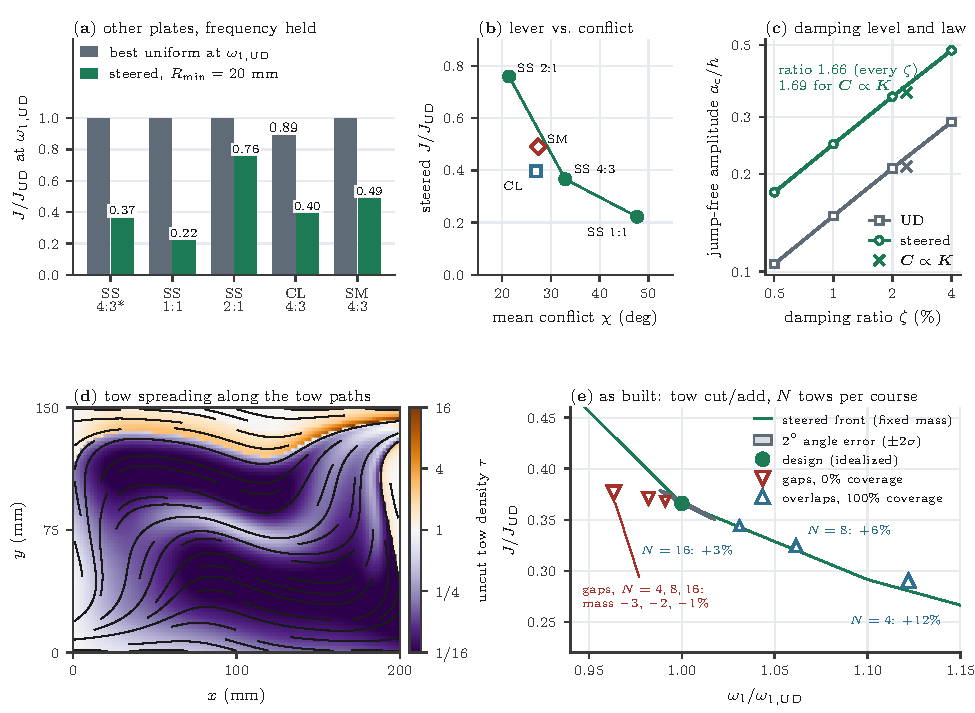
\includegraphics[width=\linewidth]{figs/fig_robust.pdf}
\caption{\textbf{The lever persists across plates, supports, damping laws and as-built defects, and its size
is ordered by the conflict between the two strain fields.} \textbf{(a)}~Held-frequency $J/J_{\UD}$ of
the steered optimum (green) and of the best uniform laminate at the same frequency (gray) for simply
supported (SS) plates of aspect ratio 4:3 (the paper's plate, $\ast$), 1:1 and 2:1, a clamped plate
(CL) and a simply supported plate with in-plane movable edges (SM). Each plate is normalized by its
own UD design; only the clamped plate has a uniform competitor other than UD at $\omega_{1,\UD}$.
\textbf{(b)}~Steered optimum vs.\ the energy-weighted conflict $\chi$ of the UD fields; line: the three
SS plates. \textbf{(c)}~Jump-free amplitude $a_c/h$ from the full damped SSM vs.\ damping ratio
(mass-proportional, lines; stiffness-proportional at $\zeta=2\%$, crosses, drawn slightly to the right for
visibility). Both designs scale as $\zeta^{1/2}$, and
their ratio does not change. \textbf{(d)}~Relative density $\tau$ of uncut constant-width tows laid
along the tow paths of the held-frequency design (black lines). Purple: spreading (gaps if uncut);
orange: convergence (overlaps); color scale clipped at $1/16$ and $16$ ($\tau$ spans
$\nTauMin$--$\nTauMax$). \textbf{(e)}~As-built laminates with tow cut/add, $N=4$, $8$, $16$ tows per course
(labels: $N$ and the mass change): resin gaps (down triangles), overlaps (up triangles), and a $2^\circ$ RMS
angle error (gray ellipse: mean $\pm2$ standard deviations). Their mass differs from UD, unlike the steered
front, which is at fixed mass.}
\label{fig:robust}
\end{figure}
